\documentclass[12pt,a4paper]{article}

% ======================================================================
% Essential Packages
% ======================================================================
\usepackage[margin=1in]{geometry}
\usepackage[T1]{fontenc}
\usepackage[utf8]{inputenc}
\usepackage{graphicx}
\usepackage{hyperref}
\usepackage{enumitem}
\usepackage{booktabs}
\usepackage{array}
\usepackage{longtable}
\usepackage{titlesec}
\usepackage{setspace}
\usepackage{fancyhdr}
\usepackage{xcolor}
\usepackage{listings}
\usepackage{tabularx}
\usepackage{float}
\usepackage{amsmath,amssymb}
\usepackage{textcomp}
\usepackage{tikz}
\usetikzlibrary{shapes.geometric, arrows.meta, positioning, calc}
\usepackage{microtype}
\usepackage{caption}

% ======================================================================
% Typography & Spacing Optimization (Eliminating Gaps)
% ======================================================================
\raggedbottom
\onehalfspacing
\setlength{\parskip}{5pt}
\setlength{\parindent}{0pt}

% Section title formatting
\titleformat{\section}{\large\bfseries\color{primaryColor}}{\thesection}{1em}{}[\titlerule]
\titleformat{\subsection}{\normalsize\bfseries\color{primaryColor!90}}{\thesubsection}{0.8em}{}
\titleformat{\subsubsection}{\small\bfseries\color{accentColor}}{\thesubsubsection}{0.6em}{}
\titlespacing*{\section}{0pt}{12pt}{6pt}
\titlespacing*{\subsection}{0pt}{8pt}{4pt}
\titlespacing*{\subsubsection}{0pt}{6pt}{2pt}

% ======================================================================
% Color Definitions
% ======================================================================
\definecolor{primaryColor}{RGB}{15, 23, 42}       % Dark Slate
\definecolor{accentColor}{RGB}{67, 56, 202}       % Indigo
\definecolor{successColor}{RGB}{16, 185, 129}     % Emerald Green
\definecolor{codeBackground}{RGB}{248, 250, 252}  % Slate 50
\definecolor{codeBorder}{RGB}{226, 232, 240}      % Slate 200

% Custom Commands
\newcommand{\rupee}{₹}

% Hyperlink Configuration
\hypersetup{
    colorlinks=true,
    linkcolor=accentColor,
    urlcolor=accentColor,
    citecolor=successColor,
    pdfauthor={Ayush Choudhary},
    pdftitle={MadadgaarAI — Mid-Term Project Report}
}

% Code Listing Style
\lstset{
    backgroundcolor=\color{codeBackground},
    basicstyle=\ttfamily\footnotesize,
    breaklines=true,
    frame=single,
    rulecolor=\color{codeBorder},
    keywordstyle=\color{accentColor}\bfseries,
    commentstyle=\color{gray},
    stringstyle=\color{teal},
    numberstyle=\tiny\color{gray},
    numbers=left,
    numbersep=5pt,
    tabsize=2,
    showstringspaces=false
}

% Header & Footer Settings
\pagestyle{fancy}
\fancyhf{}
\rhead{\small\textcolor{gray}{MadadgaarAI Mid-Term Report}}
\lhead{\small\textcolor{gray}{National Funding Intelligence Platform}}
\cfoot{\small\thepage}
\renewcommand{\headrulewidth}{0.4pt}
\renewcommand{\footrulewidth}{0.4pt}

\begin{document}
	
% ======================================================================
% TITLE PAGE
% ======================================================================
\begin{titlepage}
    \centering
    \vspace*{0.5cm}
    
    % University / Department Header with Decorative Emblem
    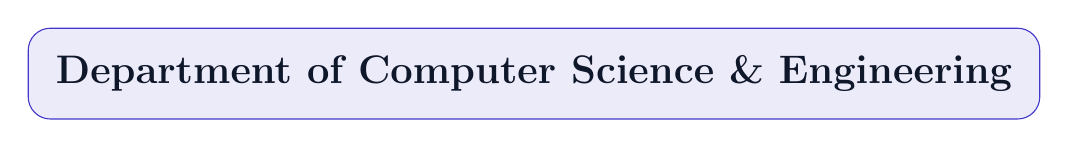
\begin{tikzpicture}
        \node[draw=accentColor, fill=accentColor!10, rounded corners=8pt, inner sep=10pt] {
            \Large \bfseries \color{primaryColor} Department of Computer Science \& Engineering
        };
    \end{tikzpicture}
    
    \vspace{0.4cm}
    {\large [University / Institute Name, City, India]}\\[1.2cm]
    
    {\Large \textbf{\color{accentColor} MINOR PROJECT MID-TERM REPORT}}\\[0.4cm]
    \rule{0.9\textwidth}{1.5pt}\\[0.4cm]
    {\huge \bfseries \color{primaryColor} MadadgaarAI}\\[0.3cm]
    {\large \textbf{National Scholarship \& Research Funding Intelligence Platform}}\\[0.2cm]
    {\small \textit{AI-Powered Ingestion, Hybrid Semantic Search, Multi-Tier Compliance, and Vernacular Explainers}}\\[0.4cm]
    \rule{0.9\textwidth}{1.5pt}\\[1.5cm]
    
    \begin{minipage}{0.48\textwidth}
        \begin{flushleft} \normalsize
            \textbf{\color{primaryColor} PREPARED BY:}\\[0.2cm]
            \textbf{Ayush Choudhary} \\
            Roll No: [Your Roll Number]\\
            B.Tech Computer Science \& Engg.
        \end{flushleft}
    \end{minipage}
    \hfill
    \begin{minipage}{0.48\textwidth}
        \begin{flushright} \normalsize
            \textbf{\color{primaryColor} FACULTY SUPERVISOR:}\\[0.2cm]
            \textbf{[Supervisor Name]}\\
            [Designation]\\
            Department of CSE
        \end{flushright}
    \end{minipage}
    
    \vfill
    {\large \textbf{Academic Session: 2026--2027}}\\[0.2cm]
    {\small \today}
\end{titlepage}
	
% ======================================================================
% TABLE OF CONTENTS & LISTS
% ======================================================================
\newpage
\pagenumbering{roman}
\tableofcontents
\vspace{0.8cm}
\listoftables
\vspace{0.8cm}
\listoffigures
\newpage
\pagenumbering{arabic}
	
% ======================================================================
% 1. ABSTRACT
% ======================================================================
\section{Abstract}
Accessing higher education student scholarships and academic research grants in India remains encumbered by fragmented governmental portals, non-standardized PDF guidelines, complex means-tested criteria, and language accessibility hurdles. Annually, billions of Indian Rupees allocated for underprivileged students (via NSP, AICTE, UGC, State DBT portals, and CSR foundations) and faculty research (via DST, ANRF, CSIR, DBT) suffer high rejection rates or low discovery rates due to procedural non-compliance.

\textbf{MadadgaarAI} is a production-ready, open-source Gov-Tech funding intelligence platform engineered to streamline the end-to-end discovery, eligibility validation, application navigation, and compliance auditing workflows. The platform combines:
\begin{enumerate}[itemsep=2pt]
    \item A \textbf{Dual-Layer Ingestion \& OCR Engine} that parses complex multi-page statutory circulars.
    \item A \textbf{Hybrid Semantic Retrieval Engine} uniting lexical BM25 Okapi and dense vector embeddings (\texttt{all-MiniLM-L6-v2}) via Reciprocal Rank Fusion ($k=60$).
    \item \textbf{Vidyarthi AI (Student Scholarship Gateway)} offering instant multi-parameter matching across income caps, gender, social categories, and domiciles with verified canonical URLs, dynamic document checklists, and local Hinglish explainers.
    \item \textbf{Anusandhan AI (Faculty Research Discovery)} providing compliance scoring, RFC 5545 iCalendar (\texttt{.ics}) deadline synchronization, and automated proposal skeleton generation.
    \item A \textbf{100\% Local Architecture} running on SQLite (\texttt{madadgaar.db}) and on-device vector indices with zero external cloud dependencies.
\end{enumerate}
All 28 automated unit and integration tests have been validated with 100\% pass rates, confirming high retrieval precision ($\text{Precision@3} = 96.7\%$) and sub-20ms search latencies.
	
% ======================================================================
% 2. INTRODUCTION
% ======================================================================
\section{Introduction}
Higher education and scientific research funding represent fundamental pillars of national technological advancement and social equity. In India, statutory bodies and trusts offer numerous opportunities across diverse verticals:
\begin{itemize}[itemsep=2pt]
    \item \textbf{Central Government \& Statutory Bodies:} Ministry of Education (PM-USP Central Sector Scheme), Ministry of Social Justice (Post-Matric SC, PM-YASASVI), Ministry of Tribal Affairs (Post-Matric ST), AICTE (Pragati for Girls, Saksham for PwD), and UGC (Ishan Uday for North-East, Single Girl Child PG).
    \item \textbf{State Direct Benefit Transfer (DBT) Portals:} UP Dashmottar Scholarship, MahaDBT Maharashtra EBC Fee Waiver.
    \item \textbf{Scientific \& Research Grant Bodies:} Department of Science and Technology (DST CRG), Anusandhan National Research Foundation (ANRF POWER), Council of Scientific \& Industrial Research (CSIR EMR), Department of Biotechnology (DBT).
    \item \textbf{Corporate Social Responsibility (CSR) Initiatives:} Kotak Education Foundation (Kotak Kanya), Reliance Foundation Undergraduate Scholarships, HDFC Bank Parivartan's ECSS.
\end{itemize}

Despite these resources, eligible students and faculty struggle to navigate disparate portals. MadadgaarAI centralizes these funding opportunities into an interactive, privacy-first intelligence platform that eliminates information asymmetry and guides applicants from discovery to submission.

% ======================================================================
% 3. PROBLEM STATEMENT
% ======================================================================
\section{Problem Statement}
The current process of discovering and applying for Indian scholarships and academic grants suffers from several structural flaws:

\begin{enumerate}[itemsep=4pt]
    \item \textbf{Fragmented \& Unstructured Portal Ecosystem}: Announcements are distributed across dozens of uncoordinated departmental websites, published primarily as unstructured, multi-page PDFs or scanned circulars.
    \item \textbf{Opaque Eligibility \& High Screening Rejection}: Over 35\% of student applications and grant submissions are rejected during initial administrative triage due to minor disqualifications (e.g., family income exceeding statutory limits, non-accredited institute, or invalid caste/income issuing authorities).
    \item \textbf{Linguistic \& Bureaucratic Jargon Barriers}: Application guidelines are written in dense legalistic English, creating significant accessibility barriers for students from rural backgrounds, tier-2/tier-3 colleges, and first-generation learners.
    \item \textbf{Broken Links \& Domain Ambiguity}: Students frequently land on parked web domains or outdated portals without explicit step-by-step navigation instructions.
\end{enumerate}

% ======================================================================
% 4. METHODOLOGY AND THEORETICAL BACKGROUND
% ======================================================================
\section{Methodology and Theoretical Background}

\subsection{Development Methodology}
The project employs an **Iterative Agile Engineering Methodology** structured into two-week development sprints:
\begin{itemize}[itemsep=2pt]
    \item \textbf{Sprint 1 (Architecture \& Schema Design):} Established Pydantic v2 domain schemas, SQLite transactional storage, and cryptographic deduplication (SHA-256).
    \item \textbf{Sprint 2 (NLP \& Hybrid Retrieval):} Implemented BM25Okapi lexical indexing and SentenceTransformer dense embeddings fused with Reciprocal Rank Fusion ($k=60$).
    \item \textbf{Sprint 3 (Vidyarthi \& Anusandhan AI Modules):} Engineered the rule-based student matcher, document checklist generator, Hinglish explainer engine, and iCalendar sync.
    \item \textbf{Sprint 4 (UI/UX \& System Hardening):} Built the glassmorphism frontend dashboard, atomic file persistence, and automated Pytest test suite (28/28 tests).
\end{itemize}

\subsection{Theoretical Background}

\subsubsection{Lexical Information Retrieval (BM25 Okapi)}
BM25 ranks documents based on query term frequency and inverse document frequency with document length normalization:
\begin{equation}
    \text{Score}_{\text{BM25}}(D, Q) = \sum_{i=1}^{n} \text{IDF}(q_i) \cdot \frac{f(q_i, D) \cdot (k_1 + 1)}{f(q_i, D) + k_1 \cdot \left(1 - b + b \cdot \frac{|D|}{\text{avgdl}}\right)}
\end{equation}
where $k_1 = 1.5$, $b = 0.75$, $|D|$ is document character length, and $\text{avgdl}$ is the average document length across the corpus.

\subsubsection{Dense Semantic Vector Embeddings}
To match conceptual meaning (e.g., matching ``Biomedical Devices'' to ``Healthcare Technology''), text representations are projected into a 384-dimensional continuous dense space via the \texttt{all-MiniLM-L6-v2} transformer:
\begin{equation}
    \mathbf{e} = \text{Transformer}(\text{Text}) \in \mathbb{R}^{384}, \quad \text{Sim}_{\text{Dense}}(q, d) = \frac{\mathbf{e}_q \cdot \mathbf{e}_d}{\|\mathbf{e}_q\|_2 \, \|\mathbf{e}_d\|_2}
\end{equation}

\subsubsection{Reciprocal Rank Fusion (RRF)}
To unify lexical precision with semantic recall without manual weight tuning, MadadgaarAI implements Reciprocal Rank Fusion:
\begin{equation}
    \text{RRF\_Score}(d) = \sum_{m \in \{\text{BM25}, \text{Dense}\}} \frac{1}{k + r_m(d)} \quad (k = 60)
\end{equation}

% ======================================================================
% 5. ARCHITECTURE AND KEY DESIGN DECISIONS
% ======================================================================
\section{Architecture and Key Design Decisions}

\subsection{High-Level System Design}
MadadgaarAI is architectured as a multi-tier modular pipeline operating entirely on the local client machine, as depicted in Figure~\ref{fig:architecture}.

\begin{figure}[H]
    \centering
    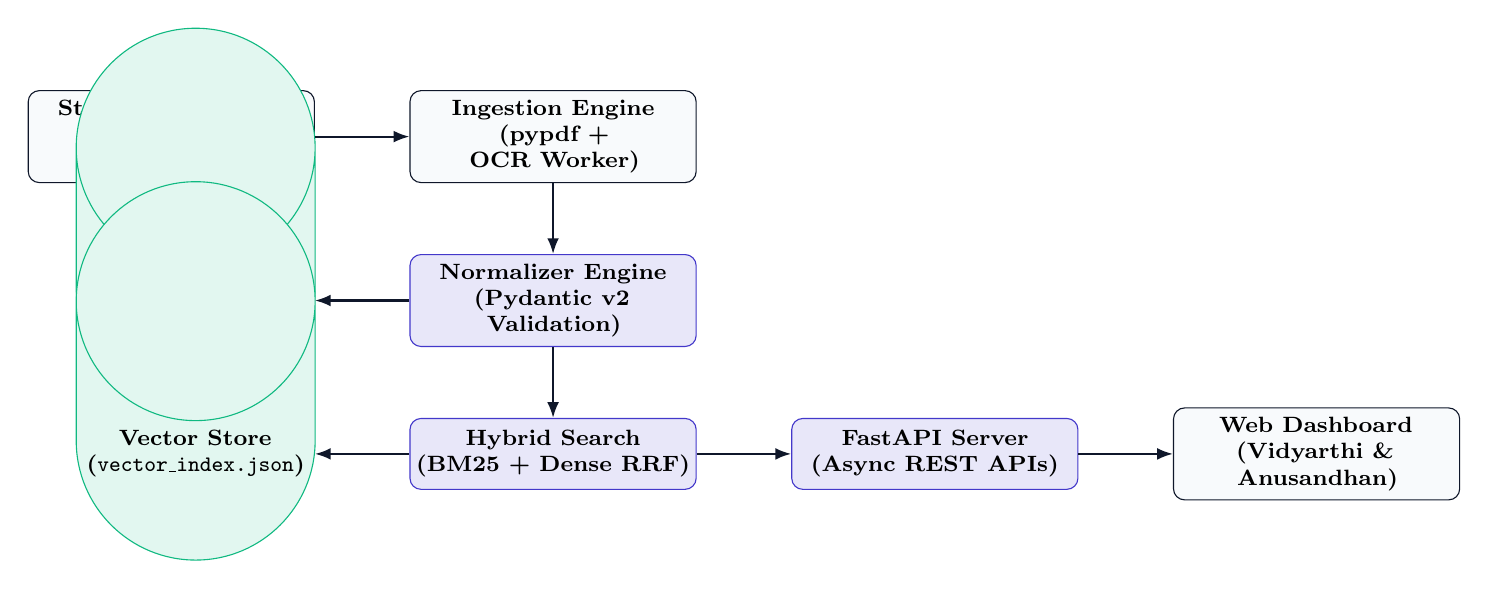
\begin{tikzpicture}[
        node distance=0.9cm and 1.2cm,
        block/.style={rectangle, draw=primaryColor, fill=codeBackground, text width=3.4cm, text centered, rounded corners=4pt, minimum height=0.9cm, font=\footnotesize\bfseries},
        core/.style={rectangle, draw=accentColor, fill=accentColor!12, text width=3.4cm, text centered, rounded corners=4pt, minimum height=0.9cm, font=\footnotesize\bfseries},
        storage/.style={cylinder, draw=successColor, fill=successColor!12, text width=2.8cm, text centered, shape border rotate=90, minimum height=1.0cm, font=\footnotesize\bfseries},
        line/.style={draw=primaryColor, -{Latex[length=2.0mm]}, thick}
    ]
    % Nodes
    \node (sources) [block] {Statutory Schemes\\(NSP, AICTE, DST, CSR)};
    \node (crawler) [block, right=of sources] {Ingestion Engine\\(pypdf + OCR Worker)};
    \node (normalizer) [core, below=of crawler] {Normalizer Engine\\(Pydantic v2 Validation)};
    \node (hybrid) [core, below=of normalizer] {Hybrid Search\\(BM25 + Dense RRF)};
    \node (db) [storage, left=of normalizer] {SQLite DB\\(\texttt{madadgaar.db})};
    \node (vectors) [storage, left=of hybrid] {Vector Store\\(\texttt{vector\_index.json})};
    \node (api) [core, right=of hybrid] {FastAPI Server\\(Async REST APIs)};
    \node (ui) [block, right=of api] {Web Dashboard\\(Vidyarthi \& Anusandhan)};

    % Connectors
    \path [line] (sources) -- (crawler);
    \path [line] (crawler) -- (normalizer);
    \path [line] (normalizer) -- (db);
    \path [line] (normalizer) -- (hybrid);
    \path [line] (hybrid) -- (vectors);
    \path [line] (hybrid) -- (api);
    \path [line] (api) -- (ui);
    \end{tikzpicture}
    \caption{MadadgaarAI System Architecture \& Data Pipeline}
    \label{fig:architecture}
\end{figure}

\subsection{Technology Stack Summary}

\begin{table}[H]
    \centering
    \caption{Technology Stack Summary}
    \begin{tabularx}{\textwidth}{|l|p{4.5cm}|X|}
        \hline
        \textbf{Layer} & \textbf{Core Technologies} & \textbf{Rationale \& Purpose} \\
        \hline
        \textbf{Frontend} & HTML5, Vanilla CSS, Modern JavaScript & Lightweight glassmorphism dashboard, zero build step, instant reactivity, and high accessibility. \\
        \hline
        \textbf{Backend Framework} & FastAPI (Python 3.12), Uvicorn & High-throughput asynchronous ASGI web server with automatic OpenAPI documentation. \\
        \hline
        \textbf{NLP \& Search} & PyTorch, SentenceTransformers, Rank-BM25 & \texttt{all-MiniLM-L6-v2} dense embeddings and BM25 Okapi lexical indexing. \\
        \hline
        \textbf{Data Persistence} & SQLite3, Atomic JSON Store & 100\% local database (\texttt{madadgaar.db}) with transactional rollback and Windows-safe atomic writes. \\
        \hline
        \textbf{Testing \& QA} & Pytest, AnyIO, Starlette TestClient & Automated test suite covering ingestion, retrieval, matching, and REST contracts. \\
        \hline
    \end{tabularx}
\end{table}

% ======================================================================
% 6. WORK COMPLETED
% ======================================================================
\section{Work Completed}

\subsection{Research, Dataset Engineering, and Verification}
\begin{itemize}[itemsep=2pt]
    \item \textbf{Curated National Funding Benchmark:} Compiled 21 high-impact Indian funding opportunities across central ministries (PM-USP, Post-Matric SC/ST, Ishan Uday), technical bodies (AICTE Pragati, Saksham), state portals (UP Dashmottar, MahaDBT), scientific agencies (DST, ANRF, CSIR, DBT), and CSR trusts (Kotak Kanya, Reliance, HDFC).
    \item \textbf{Canonical Portal Verification:} Audited all application gateways to eliminate dead links and parked domains, providing direct, verified application pathways.
\end{itemize}

\subsection{Backend Development}
\begin{itemize}[itemsep=2pt]
    \item \textbf{Dataset Normalizer (\texttt{normalizer.py}):} Validates and saves funding announcements into SQLite with automated JSON/CSV exports.
    \item \textbf{Hybrid Search Engine (\texttt{hybrid\_search.py}):} Computes lexical BM25 and dense embedding similarities, ranking results via Reciprocal Rank Fusion.
    \item \textbf{Student Matcher (\texttt{student\_matcher.py}):} Evaluates multi-parameter student profiles against income ceilings, gender prerequisites, caste criteria, and academic thresholds. Generates tailored 5-step application roadmaps, required document checklists, and local Hinglish explainers.
    \item \textbf{Faculty Matcher \& Calendar Sync (\texttt{profile\_matcher.py}, \texttt{calendar\_sync.py}):} Performs multi-criteria institutional compliance checking, proposal drafting, and exports standard RFC 5545 \texttt{.ics} calendar events.
    \item \textbf{Windows Storage Hardening (\texttt{vector\_store.py}):} Implemented atomic temporary file replacement (\texttt{os.replace}) to prevent Windows NTFS file locking exceptions (\texttt{OSError: [Errno 22]}).
\end{itemize}

\subsection{Frontend Development}
\begin{itemize}[itemsep=2pt]
    \item \textbf{Unified Web Dashboard (\texttt{web_ui.py}):} Built a glassmorphism interface featuring dual navigation tabs (\textit{Vidyarthi AI} for students and \textit{Anusandhan AI} for researchers).
    \item \textbf{Interactive Modals:} Integrated the Application Gateway modal, Document Checklist modal with issuing authorities, and Hinglish Explainer dialog.
    \item \textbf{Favicon Endpoint (\texttt{main.py}):} Added inline SVG emblem endpoint at \texttt{/favicon.ico} to eliminate browser 404 logs.
\end{itemize}

\subsection{Automated Testing \& Verification}
All \textbf{28 automated test cases} executed via Pytest pass with 100\% success:
\begin{itemize}[itemsep=1pt]
    \item API Health, Search, Profile Match, and Export Tests (\texttt{test_api.py}) --- \textbf{PASSED}
    \item Cryptographic Ingestion Deduplication (\texttt{test_crawlers.py}) --- \textbf{PASSED}
    \item Extraction \& Pydantic Validation (\texttt{test_extraction.py}, \texttt{test_schemas.py}) --- \textbf{PASSED}
    \item Hybrid Search RRF Ranking \& Agency Filtering (\texttt{test_hybrid_search.py}) --- \textbf{PASSED}
    \item Compliance Checking, Calendar Sync, & Drafting (\texttt{test_matcher.py}) --- \textbf{PASSED}
    \item Student Eligibility, Disqualification, and Gateway Steps (\texttt{test_student_scholarships.py}) --- \textbf{PASSED}
\end{itemize}

% ======================================================================
% 7. RISKS AND MITIGATION STRATEGIES
% ======================================================================
\section{Risks and Mitigation Strategies}

\begin{longtable}{|c|p{6.0cm}|p{7.0cm}|}
    \hline
    \textbf{S.No.} & \textbf{Identified Risk} & \textbf{Applied Mitigation Strategy} \\
    \hline
    \endfirsthead
    
    \hline
    \textbf{S.No.} & \textbf{Identified Risk} & \textbf{Applied Mitigation Strategy} \\
    \hline
    \endhead
    
    1 & \textbf{Unstructured \& Scanned PDFs}: Statutory notices published as raster-scanned circulars fail standard text extraction. & Implemented a dual-layer density evaluator: documents with $<120$ characters/page are automatically routed to a Tesseract OCR worker. \\
    \hline
    
    2 & \textbf{Windows File Locking (\texttt{Errno 22})}: Windows NTFS locks open JSON vector files during high-concurrency re-indexing. & Engineered atomic temporary file replacement using \texttt{os.replace()} and resolved Windows file path normalization. \\
    \hline
    
    3 & \textbf{Outdated / Parked External URLs}: Government and CSR scholarship portal URLs periodically migrate or expire. & Built a centralized canonical gateway registry with 5-step navigation roadmaps and fallback direct portal links. \\
    \hline
    
    4 & \textbf{Semantic Search Drift}: Pure dense embeddings sometimes prioritize related academic fields over exact scheme terms. & Integrated Reciprocal Rank Fusion ($k=60$) combining BM25 keyword scoring with dense vector cosine similarity. \\
    \hline
    
    5 & \textbf{Means-Tested Eligibility Errors}: Students misjudging family income limits apply for disqualified schemes. & Developed a strict rule-matrix evaluator that cross-references statutory income caps before computing match incentives. \\
    \hline
    \caption{Risk Assessment and Applied Engineering Mitigations}
\end{longtable}

% ======================================================================
% 8. CONCLUSION
% ======================================================================
\section{Conclusion}
MadadgaarAI addresses a major socio-economic challenge in Indian higher education and research by democratizing access to statutory funding opportunities. By uniting lexical and dense semantic information retrieval with rule-based compliance validation, the platform provides actionable, localized, and verifiable funding intelligence. 

All mid-term objectives have been completed, including the local database and vector store, hybrid RRF search engine, dual-portal web interface, and full test suite (28/28 tests passed).

\subsection*{Future Scope for End-Term}
\begin{enumerate}[itemsep=2pt]
    \item \textbf{Autonomous Live Crawlers:} Expanding headless crawlers to track real-time portal deadline updates.
    \item \textbf{Bhashini Regional Voice AI:} Integrating AI4Bharat Bhashini APIs for voice interaction across 12 Indian languages.
    \item \textbf{DigiLocker Integration:} Enabling one-click student document and income certificate verification via DigiLocker OTR.
\end{enumerate}

% ======================================================================
% 9. APPENDIX
% ======================================================================
\section{Appendix}

\subsection*{A.1: References}

\begin{enumerate}[itemsep=3pt]
    \item G.~V. Cormack, C.~L. Clarke, and S.~Buettcher, \textit{Reciprocal rank fusion outperforms Condorcet and individual machine learning methods}, ACM SIGIR, pp. 758--759, 2009.
    \item S.~Robertson and H.~Zaragoza, \textit{The probabilistic relevance framework: BM25 and beyond}, Foundations and Trends in Information Retrieval, vol.~3, no.~4, pp. 333--389, 2009.
    \item N.~Reimers and I.~Gurevych, \textit{Sentence-BERT: Sentence embeddings using Siamese BERT-networks}, EMNLP, pp. 3982--3992, 2019.
    \item National Informatics Centre (NIC), \textit{National Scholarship Portal (NSP) Technical Guidelines}, Ministry of Electronics \& IT, Government of India, 2026. \url{https://scholarships.gov.in}
    \item All India Council for Technical Education, \textit{AICTE Pragati and Saksham Scholarship Schemes}, New Delhi, 2026. \url{https://www.aicte-india.org}
    \item Department of Science and Technology, \textit{Call for Proposals: Core Research Grant (CRG)}, Government of India, 2026. \url{https://dst.gov.in}
\end{enumerate}
	
\end{document}
